\chapter{Classificação de Qualidade de Superfície de Pista}
\label{cap:classificacao_qualidade}

Nesta seção é apresentado o estudo, desenvolvimento e experimentação voltado ao desenvolvimento de um modelo adaptativo para classificação da qualidade de superfície da pista. Baseado nos resultados dos experimentos das seções anteriores, este estudo focou no desenvolvimento de modelos baseados em \textit{Deep Learning}. O processo de desenvolvimento e experimentação é detalhado nas próximas subseções. Na primeira delas, de pré-processamento, foi realizada a seleção de variáveis, padronizados seus dados através de normalização dos sinais, e definidos experimentos para avaliar aspectos como ponto de coleta de dados no veículo, tamanho da janela de dados e variações contextuais, onde foi possível analisar a capacidade de generalização do aprendizado dos modelos para contextos desconhecidos e, portanto, avaliar sua adaptabilidade. Na segunda subseção, de processamento, foram desenvolvidos cinco modelos de DNN baseados em diferentes técnicas de \textit{Deep Learning}: LSTM, GRU, CNN, CNN-LSTM e ConvLSTM. Por fim, na última subseção são detalhados e comparados os resultados obtidos.

\section{Pré-Processamento}

Com base nos resultados obtidos nos experimentos anteriores, neste estudo utilizamos como características de entrada os dados brutos das variáveis de aceleração em três eixos (X, Y, Z) e em três diferentes pontos de coleta (abaixo e próximo da suspensão, acima e próximo da suspensão e painel de controle), juntamente com os dados de taxa rotação em três eixos e em três diferentes pontos de coleta, além da velocidade do veículo. Inicialmente, todos os dados foram normalizados com \textit{Robust Scaler}, o qual utilizando intervalo interquartil se mostra um escalador mais robusto para dados com \textit{outliers} \cite{Vaitheeshwari2019}. Os dados das características foram normalizados mantendo o sinal, uma vez que o sinal contém informação importante de direção do vetor de força. Após a normalização dos dados, para avaliar a influência da propriedade de dependência veicular e verificar a viabilidade de um modelo de classificação para os dados coletados em diferentes pontos do veículo, foram definidos os seguintes \emph{experimentos por colocação}, com base nos pontos de coleta de dados no veículo:

\begin{description}
	
	\item[Experimento por Colocação 1:] Foram utilizados os dados de força de aceleração 3D e taxa de rotação 3D amostrados próximo e abaixo da suspensão, mais a velocidade.
    
    \item[Experimento por Colocação 2:] Foram utilizados os dados de força de aceleração 3D e taxa de rotação 3D amostrados próximo e acima da suspensão, mais a velocidade.
    
    \item[Experimento por Colocação 3:] Foram utilizados os dados de força de aceleração 3D e taxa de rotação 3D amostrados no painel de controle, mais a velocidade.
    
\end{description}

Para avaliar a capacidade de generalização do aprendizado de cada técnica, avaliando sua adaptabilidade para contextos desconhecidos onde há variação nas propriedades de dependência veicular, de condução e ambiental, os dados de treinamento e validação foram divididos da mesma maneira que as pesquisas das seções anteriores, separando-os de acordo com o conjunto de dados em três \emph{experimentos por contexto}:

\begin{description}
	
	\item[Experimento por Contexto 1:] O modelo aprende dados de todos os veículos e motoristas para alguns cenários; mas não todos os veículos com todos os motoristas para todos os cenários.
    \begin{itemize}
        \item \textbf{Treinamento (65\%):} PVS 1, PVS 3, PVS 4, PVS 6, PVS 7, PVS 9. 
        \item \textbf{Validação (35\%):} PVS 2, PVS 5, PVS 8.
    \end{itemize}
    
    \item[Experimento por Contexto 2:] O modelo aprende dados de todos os cenários para alguns veículos e alguns motoristas; mas não todos os veículos com todos os motoristas para todos os cenários.
    \begin{itemize}
        \item \textbf{Treinamento (66\%):} PVS 1, PVS 2, PVS 3, PVS 7, PVS 8, PVS 9.
        \item \textbf{Validação (34\%):} PVS 4, PVS 5, PVS 6.
    \end{itemize}
    
    \item[Experimento por Contexto 3:] O modelo aprende dados de alguns veículos com alguns motoristas para alguns cenários; mas não todos os veículos com todos os motoristas para todos os cenários.
    \begin{itemize}
        \item \textbf{Treinamento (66\%):} PVS 1, PVS 2, PVS 4, PVS 6, PVS 8, PVS 9.
        \item \textbf{Validação (34\%):} PVS 3, PVS 5, PVS 7.
    \end{itemize}
    
\end{description}

Finalmente, para analisar a influência do número de amostras na classificação, foram criados três \emph{experimentos por tamanho de janela de dados}, com janelas de 100, 200, 300, 400, e 500 amostras. A janela de dados utilizada foi fixa sem sobreposição, e cada amostra correspondeu a um vetor com os valores das características. Em resumo, cada experimento realizado neste estudo é um elemento do produto cartesiano entre \emph{experimentos por colocação}, \emph{experimentos por contexto} e \emph{experimentos por tamanho de janela de dados}, conforme ilustra a \autoref{fig:combinacao_experimentos_3}.

\begin{figure}[h]
  \centering
  \caption{Combinação de tipos de experimentos}
  \label{fig:combinacao_experimentos_3}
  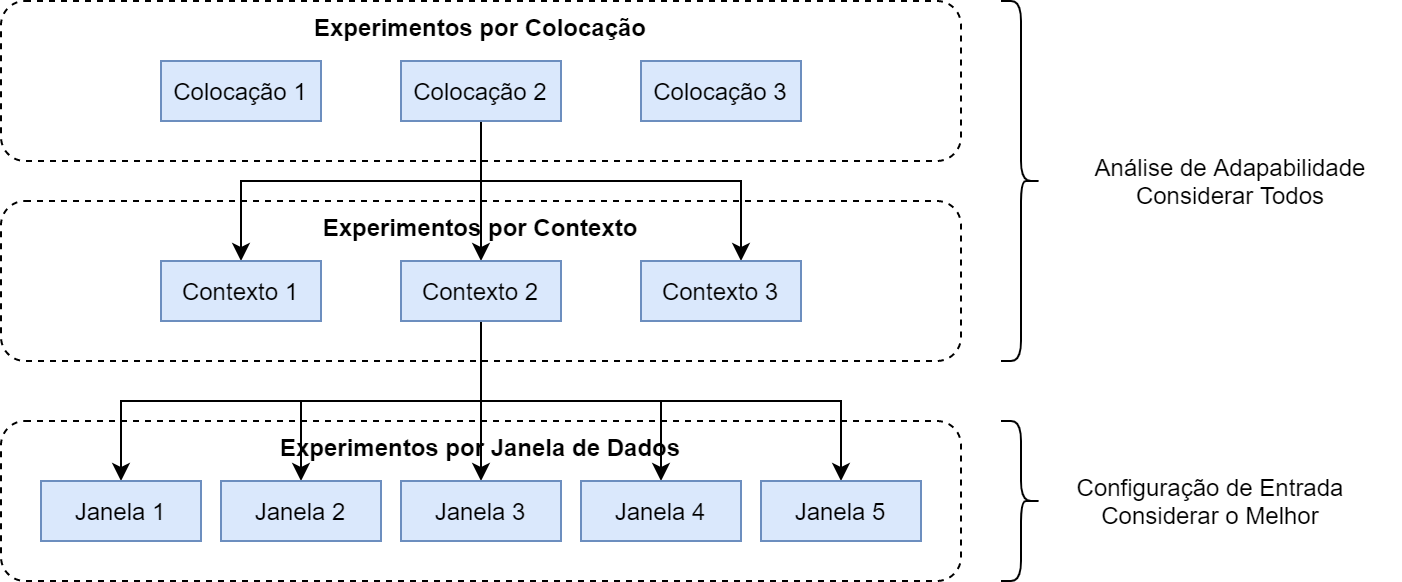
\includegraphics[width=1\textwidth]{figuras/fig_45_1.png}
  \fonte{Desenvolvido pelo autor.}
\end{figure}

Para avaliar a necessidade de aplicar técnicas de balanceamento de classe de dados, foi medida a distribuição de cada classe conforme detalhado na \autoref{table:distribuicao_classes_qualidade_superficie}. A distribuição de classes foi calculada com os dados de treinamento \cite{He2013,Kuhn2013}, uma vez que estes são os dados utilizados pelos modelos para aprender os padrões. A distribuição foi calculada em relação ao número de amostras, uma vez que as janelas de dados são definidas de acordo com esse parâmetro. Analisando a \autoref{table:distribuicao_classes_qualidade_superficie}, observamos que a distribuição das classes de qualidade de superfície de pista situa-se entre 10,58\% e 47,73\%, dependendo do experimento. A proporção varia entre 1:1,1 a 1:8,5, onde para 1 amostra de uma determinada classe de dados, existem de 1,1 a 8,5 amostras nas outras classes. O desbalanceamento de classes pode ser considerado leve ou severo, onde as proporções de distribuição que variam de 1:4 até 1:100 (presença de 20\% - 1\%) são consideradas desbalanceamento leve e proporções de distribuição que variam de 1:100 ou mais (<1\% de presença) são consideradas desbalanceamentos severos \cite{Krawczyk2016,Brownlee2020}. Como podemos observar, as proporções de distribuição das classes de dados neste estudo em sua maioria não são classificadas sequer como desbalanceamento leve, e os poucos que são desbalanceamento leve, não há tendência a desbalanceamento severo. Sendo assim, este estudo não necessita de aplicação de técnica para balanceamento de classes. Com a definição dos experimentos, convêm ressaltar a diferença entre o modelo de GT de anotação automatizada por máquina e o modelo que se busca obter com estes experimentos. No primeiro, os três modelos de KMC gerados estão cada um deles em função de um dos veículos. Já neste estudo, os experimentos buscam por um único modelo que se adapte aos três veículos.

\begin{table}[h]
\caption{Distribuição de classes de dados de qualidade de superfície de pista}
\label{table:distribuicao_classes_qualidade_superficie}
\centering
\scriptsize
\begin{tabular}{lcccccc}
\cmidrule(l){2-7}
\multicolumn{1}{c}{\multirow{2}{*}{\textbf{}}} & 
\multicolumn{6}{c}{\textbf{Classe de Dados}} \\ \cmidrule(l){2-7} 
\multicolumn{1}{c}{} & 
\multicolumn{2}{c}{\textbf{Bom}} & 
\multicolumn{2}{c}{\textbf{Regular}} & 
\multicolumn{2}{c}{\textbf{Ruim}} \\ \midrule
\textbf{Fonte de Dados} & 
\textit{\textbf{Percentual}} & 
\textit{\textbf{Proporção}} & 
\textit{\textbf{Percentual}} & 
\textit{\textbf{Proporção}} & 
\textit{\textbf{Percentual}} & 
\textit{\textbf{Proporção}} \\ \midrule
Exp. por Contexto 1 & 41,69\% & 1:1,4 & 47,73\% & 1:1,1 & 10,58\% & 1:8,5 \\ \midrule
Exp. por Contexto 2 & 43,53\% & 1:1,3 & 40,17\% & 1:1,5 & 16,30\% & 1:5,1 \\ \midrule
Exp. por Contexto 3 & 42,51\% & 1:1,4 & 40,64\% & 1:1,5 & 16,85\% & 1:4,9 \\ \bottomrule
\end{tabular}
\fonte{Desenvolvido pelo autor.}
\end{table}

\section{Processamento}

Após o pré-processamento, os dados foram aplicados em cinco modelos de \textit{Deep Learning}, sendo baseados em LSTM, GRU, CNN, CNN-LSTM e ConvLSTM. Todos os modelos desenvolvidos são sequenciais e utilizam o otimizador Adam em conjunto com a função de perda Entropia Cruzada Categórica. Todos os modelos tiveram seus hiperparâmetros ajustados (\textit{hyperparameter tuning}) utilizando o algoritmo \textit{HyperBand} implementado na biblioteca Keras Tuner, onde foram testados diferentes tipos de camadas, número de camadas e neurônios, funções de ativação e várias outras características para encontrar o conjunto ideal de hiperparâmetros para cada DNN. 

O melhor modelo baseado em LSTM obtido através do ajuste de hiperparâmetros é detalhado na \autoref{fig:best_lstm_qualidade_superficie}. O modelo DNN é composto de um bloco de camada de entrada, três blocos de camadas de recorrência e regularização e três blocos de camada totalmente conectadas para produção da saída. O bloco de entrada possui uma camada que recebe um tensor \emph{janelas x sequências x características}, onde \emph{janelas} são os agrupamentos de todas as janelas de dados, \emph{sequências} são as sequências de dados para cada janela, e \emph{características} são os valores das variáveis de entrada. Cada bloco de recorrência e regularização é composto por uma camada LSTM unidirecional de 64 unidades, seguida por uma camada de \textit{Batch Normalization} e uma camada de \textit{Dropout} em 35\%. Após o processamento nas camadas recorrentes, os parâmetros são passados para os blocos totalmente conectados, onde existem duas camadas \textit{Dense} com 160 neurônios e ativação \textit{Sigmoid}, e uma camada \textit{Dense} com 3 neurônios e ativação \textit{Softmax}, produzindo a classificação. A saída esperada são os rótulos mais presentes na janela de dados.

\begin{figure}[h!]
  \centering
  \caption{Modelo LSTM para classificação de qualidade de superfície de pista}
  \label{fig:best_lstm_qualidade_superficie}
  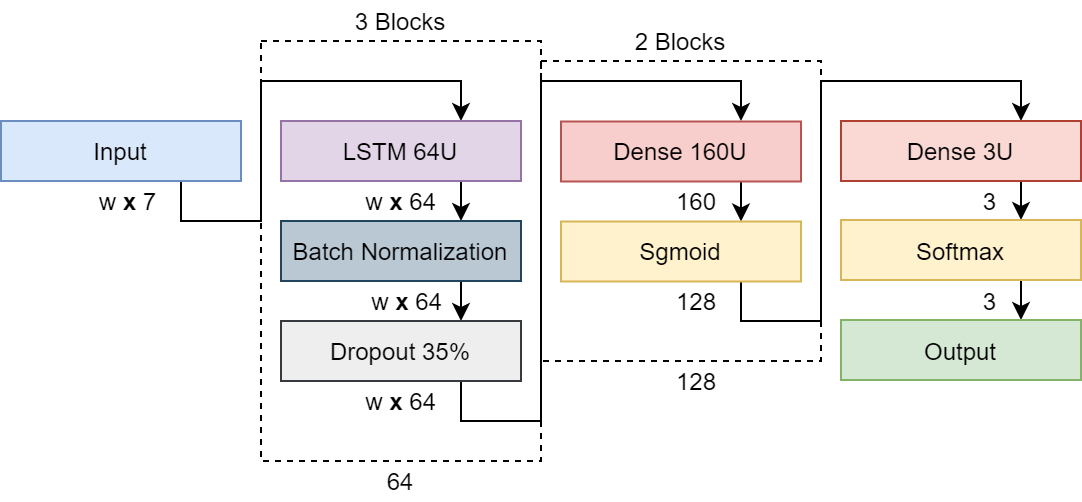
\includegraphics[width=0.7\textwidth]{figuras/fig_46.png}
 \fonte{Desenvolvido pelo autor.}
\end{figure}

O melhor modelo baseado em GRU obtido neste estudo é detalhado na \autoref{fig:best_gru_qualidade_superficie}. O modelo de DNN é composto de um bloco de camada de entrada, três blocos de camadas de recorrência e regularização e um bloco de camadas totalmente conectadas para produção de saída. O bloco de entrada possui uma camada que recebe um tensor \emph{janelas x sequências x características}, semelhante ao baseado em LSTM. Cada bloco de recorrência e regularização é composto por uma camada GRU unidirecional de 32 unidades, seguida por uma camada de \textit{Batch Normalization} e uma camada de \textit{Dropout} em 50\%. Após o processamento nas camadas recorrentes, os parâmetros passam para um bloco totalmente conectado, onde existe uma camada \textit{Dense} com 3 neurônios e ativação \textit{Softmax}, produzindo a classificação.

\begin{figure}[h!]
  \centering
  \caption{Modelo GRU para classificação de qualidade de superfície de pista}
  \label{fig:best_gru_qualidade_superficie}
  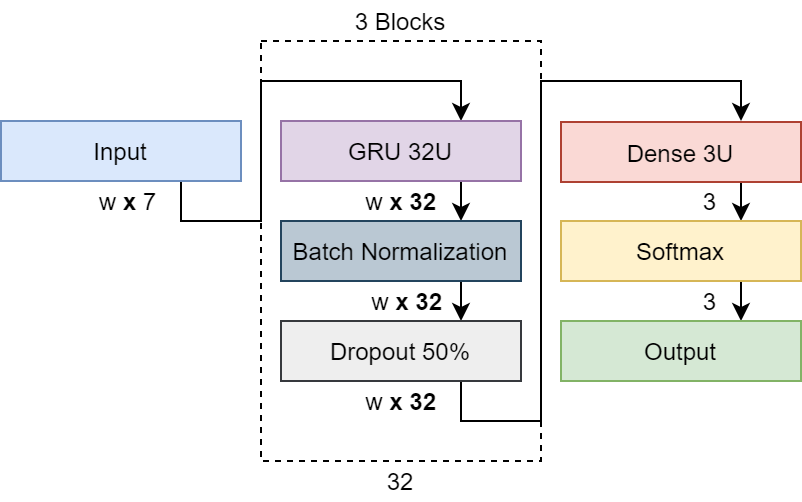
\includegraphics[width=0.5\textwidth]{figuras/fig_47.png}
 \fonte{Desenvolvido pelo autor.}
\end{figure}

O melhor modelo baseado em CNN obtido é detalhado na \autoref{fig:best_cnn_qualidade_superficie}. O modelo de DNN é composto de um bloco de entrada, dois blocos de convolução e regularização e um bloco de camadas totalmente conectadas para produção de saída. O bloco de entrada possui uma camada que recebe um tensor \emph{janelas x sequências x características}, semelhante aos modelos baseados em LSTM e GRU. O primeiro bloco de convolução e regularização é composto por uma camada Conv 1D com 224 filtros com \textit{kernel} de tamanho 7 para extração de características e ativação \textit{Relu}, seguida de regularização através de uma camada de \textit{Batch Normalization} e uma camada de \textit{Spatial Dropout 1D} em 50\%. O último bloco de convolução e regularização tem uma camada Conv 1D com as mesmas configurações do anterior, uma camada \textit{Global Max Pooling 1D} para extrair recursos mais robustos por meio dos valores máximos em cada região, e camadas de regularização por \textit{Batch Normalization 1D} e \textit{Dropout} em 40\%. Finalmente, o bloco totalmente conectado consiste de uma camada \textit{Dense} com 3 neurônios e ativação \textit{Softmax}, produzindo a classificação.

\begin{figure}[h!]
  \centering
  \caption{Modelo CNN para classificação de qualidade de superfície de pista}
  \label{fig:best_cnn_qualidade_superficie}
  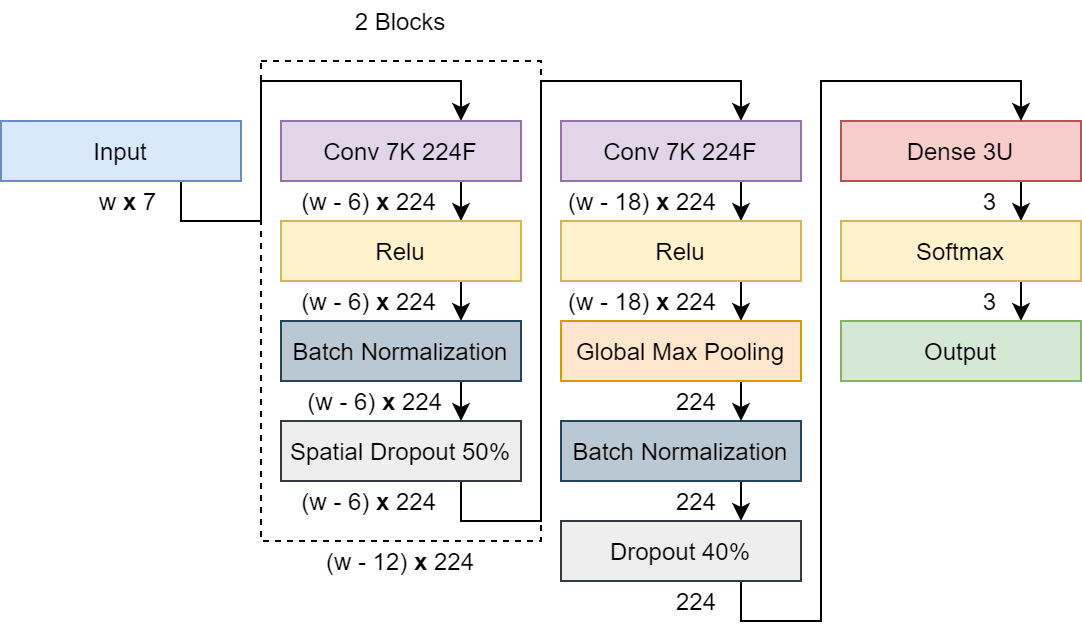
\includegraphics[width=0.7\textwidth]{figuras/fig_48.png}
 \fonte{Desenvolvido pelo autor.}
\end{figure}

O melhor modelo híbrido baseado em CNN-LSTM obtido é detalhado na \autoref{fig:best_cnn_lstm_qualidade_superficie}. O modelo de DNN é composto de um bloco de entrada, dois blocos de convolução e regularização, dois blocos recorrentes e de regularização e dois blocos de camada totalmente conectadas para produção de saída. O bloco de entrada tem uma camada que recebe um tensor \emph{janelas x sequências x subsequências x características}, onde \emph{janelas} são os agrupamentos de todas as janelas de dados, \emph{sequências} são as sequências de dados para cada janela, \emph{subsequências} são as subpartes da sequência de dados original, e \emph{características} os valores das variáveis de entrada. O primeiro bloco de convolução e regularização é composto por uma camada Conv 1D com 64 filtros com \textit{kernel} de tamanho 3 para extração de características e ativação \textit{Relu}, seguida de regularização através de uma camada de \textit{Batch Normalization} e uma camada de \textit{Spatial Dropout 1D} em 15\%. O último bloco de convolução e regularização tem uma camada Conv 1D com as mesmas configurações do anterior, uma camada \textit{Global Average Pooling 1D} para extrair recursos mais robustos por meio da média dos valores em cada região, uma camada \textit{Flatten} para reagrupar os recursos extraídos na sequência temporal original, e regularização por camada de \textit{Batch Normalization}. Em seguida, cada bloco de recorrência e regularização é composto por uma camada LSTM unidirecional de 64 unidades, seguida por uma camada de \textit{Batch Normalization} e uma camada de \textit{Dropout} em 45\%. Finalmente, os parâmetros resultantes passam para duas camadas \textit{Dense}, a primeira com 128 neurônios e ativação de \textit{Relu}, e a segunda com 3 neurônios e ativação de \textit{Softmax}, produzindo a classificação. 

\begin{figure}[h!]
  \centering
  \caption{Modelo CNN-LSTM para classificação de qualidade de superfície de pista}
  \label{fig:best_cnn_lstm_qualidade_superficie}
  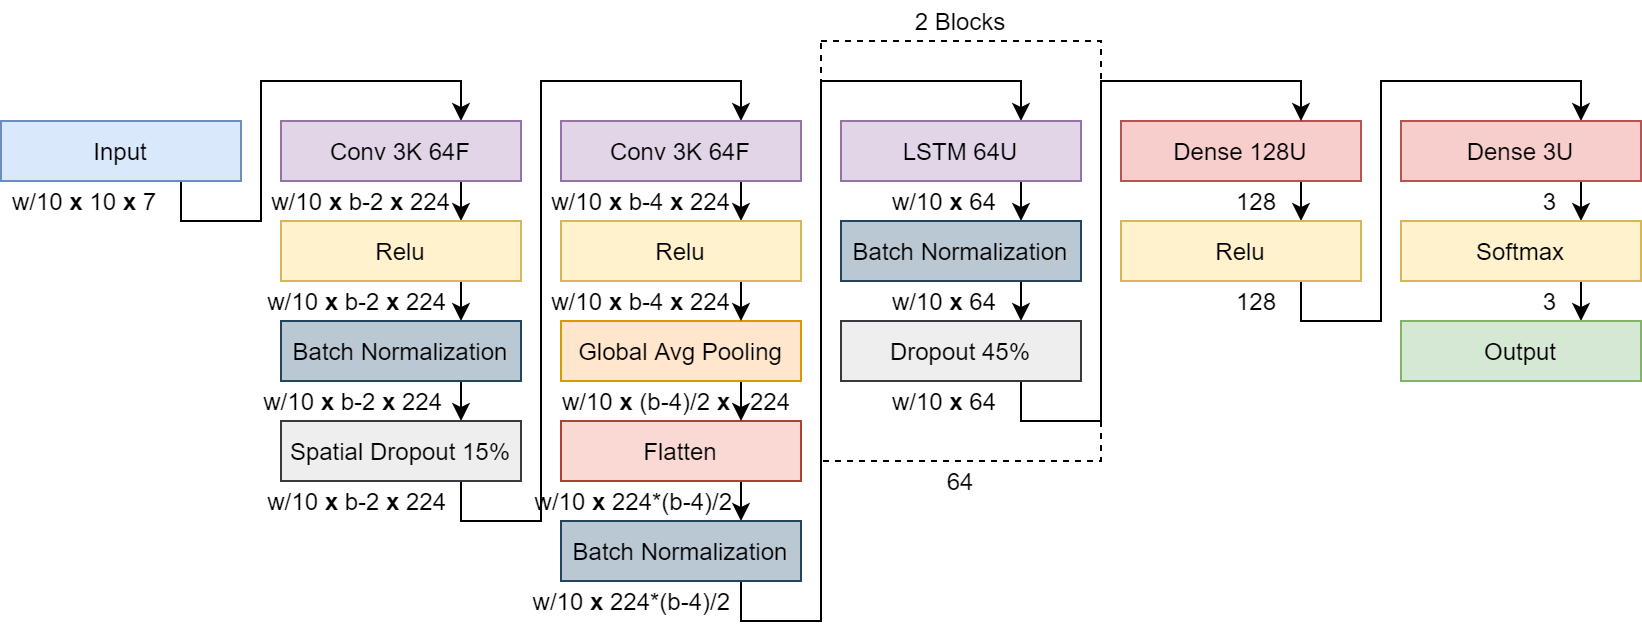
\includegraphics[width=1\textwidth]{figuras/fig_49.png}
 \fonte{Desenvolvido pelo autor.}
\end{figure}

O melhor modelo baseado em ConvLSTM obtido é detalhado na Figura \autoref{fig:best_conv_lstm_qualidade_superficie}. O modelo de DNN é composto de um bloco de entrada, um bloco convolucional recorrente e de regularização, e dois blocos de camadas totalmente conectadas para produção de saída. O bloco de entrada possui uma camada que recebe um tensor \emph{janelas x sequências x subsequências x características}, semelhante ao modelo CNN-LSTM. O bloco convolucional recorrente e de regularização é composto por uma camada \textit{ConvLSTM 1D} com 224 filtros \textit{kernel} de tamanho 7 e ativação \textit{Relu}, seguido por regularização através de uma camada \textit{Dropout} em 35\%. Finalmente, os parâmetros resultantes são achatados (\textit{flattened)} e passados para duas camadas \textit{Dense}, a primeira com 160 neurônios e ativação \textit{Relu}, e a segunda com 3 neurônios e ativação \textit{Softmax}, produzindo a classificação.

\begin{figure}[ht!]
  \centering
  \caption{Modelo ConvLSTM para classificação de qualidade de superfície de pista}
  \label{fig:best_conv_lstm_qualidade_superficie}
  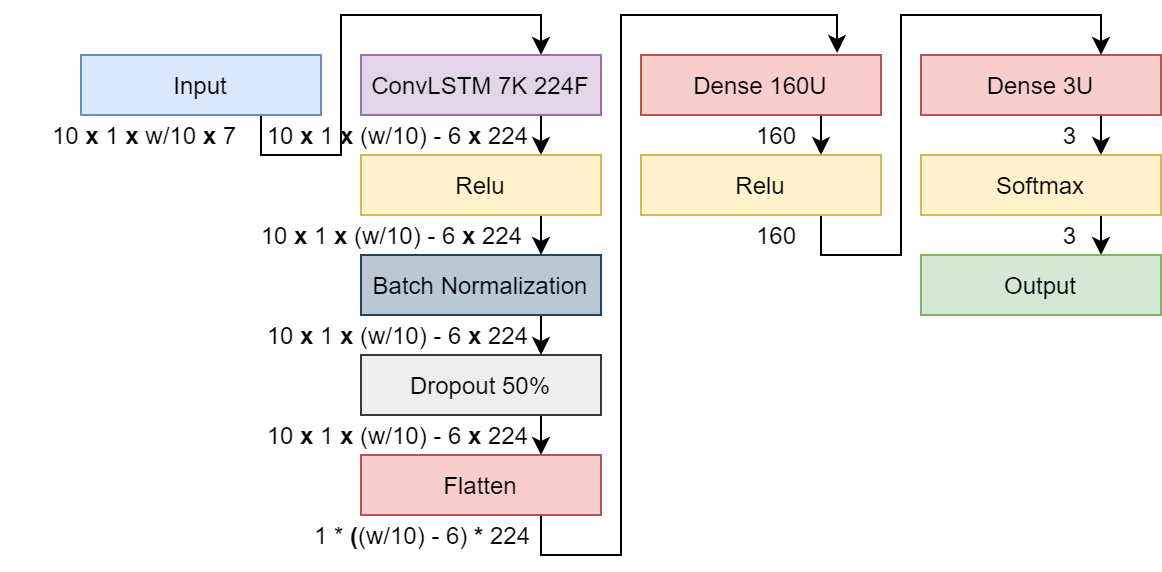
\includegraphics[width=0.7\textwidth]{figuras/fig_50.png}
 \fonte{Desenvolvido pelo autor.}
\end{figure}

Os demais hiperparâmetros das técnicas de \textit{Deep Learning} foram utilizados com seus valores padrões, disponíveis em \citeonline{tensorflow1}, \citeonline{tensorflow2}, \citeonline{tensorflow3} e \citeonline{tensorflow4}.

\section{Análise de Resultados}

Neste estudo todos os modelos de classificação de qualidade de superfície foram desenvolvidos na linguagem Python 3, utilizando da biblioteca Keras 2, a qual é uma API de alto nível do TensorFlow. Os hiperparâmetros dos modelos foram afinados através da biblioteca Keras Tuner. Todos os experimentos foram executados em máquinas do Google \textit{Collaboratory}, com as mesmas configurações dos estudos das seções anteriores. Todas as configurações de treinamento estão detalhadas nos códigos-fonte documentados disponíveis na página do projeto no Github. Cada experimento executado é um elemento do produto Cartesiano entre \emph{experimentos por colocação}, \emph{experimentos por contexto} e \emph{experimentos por tamanho da janela de dados}. Cada experimento foi executado três vezes, para minimizar a aleatoriedade de parâmetros iniciais, como pesos sinápticos, recuperando-se o melhor das três execuções. Consideramos a melhor execução aquele com maior valor de acurácia na fase de validação, uma vez que o treinamento dos modelos foi configurado para maximizar a métrica de acurácia.

Os resultados obtidos com a execução de todos os experimentos são apresentados nas Tabelas \ref{table:lstm_accuracy_result_qualidade_superficie} a \ref{table:conv_lstm_accuracy_result_qualidade_superficie}. Em cada tabela são detalhados os resultados para determinado modelo de DNN, para cada colocação, contexto e janela de dados. Também são apresentadas métricas de média aritmética para cada tipo de experimento, sendo Acurácia Média dos Experimentos por Contexto (AMEC) e Acurácia Média dos Experimentos por Contexto e Colocação (AMECC), onde são destacados os menores e maiores valores de acurácia obtidos na fase de validação.

\begin{table}[H]
\scriptsize
\centering
\caption{Valores de acurácia em validação obtidos pelo modelo LSTM} 
\label{table:lstm_accuracy_result_qualidade_superficie}
\begin{tabular}{ccccccc}
\toprule
\multicolumn{2}{c}{\textbf{Tipo de Experimento}} & \multicolumn{5}{c}{\textit{\textbf{Tamanho da Janela de Dados}}} \\ \midrule
\textit{\textbf{Colocação}} & \textit{\textbf{Contexto}} & \textit{100} & \textit{200} & \textit{300} & \textit{400} & \textit{500} \\ \midrule
\multirow{4}{*}{\begin{tabular}[c]{@{}c@{}} \\ Próximo e Abaixo \\ da Suspensão\end{tabular}} 
& 1 & 89,79\% & 90,89\% & 91,40\% & 91,67\% & 91,61\% \\ \cmidrule(l){2-7} 
& 2 & 90,37\% & 91,31\% & 93,00\% & 92,49\% & 90,94\% \\ \cmidrule(l){2-7} 
& 3 & 91,42\% & 92,20\% & 92,90\% & 92,00\% & 92,99\% \\ \cmidrule(l){2-7} 
& AMEC & \cellcolor[HTML]{FFCCC9}90,53\% & 91,47\% & \cellcolor[HTML]{34FF34}92,43\% & 92,05\% & 91,85\% \\ \midrule
\multirow{4}{*}{\begin{tabular}[c]{@{}c@{}} \\ Próximo e Acima \\ da Suspensão\end{tabular}} 
& 1 & 90,14\% & 91,10\% & 92,42\% & 92,03\% & 91,55\% \\ \cmidrule(l){2-7} 
& 2 & 90,63\% & 92,11\% & 92,34\% & 92,27\% & 91,42\% \\ \cmidrule(l){2-7} 
& 3 & 91,54\% & 92,26\% & 92,50\% & 93,04\% & 91,56\% \\ \cmidrule(l){2-7} 
& AMEC & \cellcolor[HTML]{FFCCC9}90,77\% & 91,82\% & 92,42\% & \cellcolor[HTML]{34FF34}92,44\% & 91,51\% \\ \midrule
\multirow{4}{*}{\begin{tabular}[c]{@{}c@{}} \\ Painel de Controle \end{tabular}} 
& 1 & 90,45\% & 90,60\% & 92,50\% & 89,83\% & 88,86\% \\ \cmidrule(l){2-7} 
& 2 & 87,96\% & 88,36\% & 91,55\% & 90,39\% & 90,11\% \\ \cmidrule(l){2-7} 
& 3 & 91,46\% & 91,68\% & 92,09\% & 92,71\% & 92,31\% \\ \cmidrule(l){2-7} 
& AMEC & \cellcolor[HTML]{FFCCC9}89,95\% & 90,21\% & \cellcolor[HTML]{34FF34}92,05\% & 90,98\% & 90,43\% \\ \midrule
& AMECC & \cellcolor[HTML]{FFCCC9}90,42\% & 91,17\% & \cellcolor[HTML]{34FF34}92,30\% & 91,82\% & 91,26\% \\ \cmidrule(l){2-7} 
\end{tabular}
\fonte{Desenvolvido pelo autor.}
\end{table}

\begin{table}[H]
\scriptsize
\centering
\caption{Valores de acurácia em validação obtidos pelo modelo GRU} 
\label{table:gru_accuracy_result_qualidade_superficie}
\begin{tabular}{ccccccc}
\toprule
\multicolumn{2}{c}{\textbf{Tipo de Experimento}} & \multicolumn{5}{c}{\textit{\textbf{Tamanho da Janela de Dados}}} \\ \midrule
\textit{\textbf{Colocação}} & \textit{\textbf{Contexto}} & \textit{100} & \textit{200} & \textit{300} & \textit{400} & \textit{500} \\ \midrule
\multirow{4}{*}{\begin{tabular}[c]{@{}c@{}} \\ Próximo e Abaixo \\ da Suspensão\end{tabular}} 
& 1 & 90,27\% & 91,20\% & 92,26\% & 91,61\% & 92,73\%  \\ \cmidrule{2-7}
& 2 & 90,89\% & 92,08\% & 92,75\% & 92,21\% & 91,98\%  \\ \cmidrule{2-7}
& 3 & 91,47\% & 92,34\% & 92,99\% & 92,87\% & 92,99\%  \\ \cmidrule{2-7}
& AMEC &  \cellcolor[HTML]{FFCCC9}90,88\% & 91,87\% & \cellcolor[HTML]{34FF34}92,67\% & 92,23\% & 92,57\%  \\ \midrule
\multirow{4}{*}{\begin{tabular}[c]{@{}c@{}} \\ Próximo e Acima \\ da Suspensão\end{tabular}} 
& 1 & 90,31\% & 92,38\% & 92,77\% & 92,82\% & 93,38\%  \\ \cmidrule{2-7}
& 2 & 90,40\% & 92,00\% & 93,41\% & 93,04\% & 92,25\%  \\ \cmidrule{2-7}
& 3 & 91,84\% & 92,83\% & 93,15\% & 92,93\% & 93,20\%  \\ \cmidrule{2-7}
& AMEC &  \cellcolor[HTML]{FFCCC9}90,85\% & 92,40\% & \cellcolor[HTML]{34FF34}93,11\% & 92,93\% & 92,94\%  \\ \midrule
\multirow{4}{*}{\begin{tabular}[c]{@{}c@{}} \\ Painel de Controle \end{tabular}} 
& 1 & 91,14\% & 91,91\% & 93,60\% & 92,66\% & 92,92\%  \\ \cmidrule{2-7}
& 2 & 90,56\% & 89,85\% & 87,74\% & 88,07\% & 86,93\%  \\ \cmidrule{2-7}
& 3 & 91,65\% & 92,69\% & 93,76\% & 94,67\% & 93,06\%  \\ \cmidrule{2-7}
& AMEC &  91,12\% & 91,48\% & 91,70\% & \cellcolor[HTML]{34FF34}91,80\% & \cellcolor[HTML]{FFCCC9}90,97\%  \\ \midrule
& AMECC  & \cellcolor[HTML]{FFCCC9}90,95\% & 91,92\% & \cellcolor[HTML]{34FF34}92,49\% & 92,32\% & 92,16\% \\ \cmidrule(l){2-7} 
\end{tabular}
\fonte{Desenvolvido pelo autor.}
\end{table}

\begin{table}[H]
\scriptsize
\centering
\caption{Valores de acurácia em validação obtidos pelo modelo CNN} 
\label{table:cnn_accuracy_result_qualidade_superficie}
\begin{tabular}{ccccccc}
\toprule
\multicolumn{2}{c}{\textbf{Tipo de Experimento}} & \multicolumn{5}{c}{\textit{\textbf{Tamanho da Janela de Dados}}} \\ \midrule
\textit{\textbf{Colocação}} & \textit{\textbf{Contexto}} & \textit{100} & \textit{200} & \textit{300} & \textit{400} & \textit{500} \\ \midrule
\multirow{4}{*}{\begin{tabular}[c]{@{}c@{}} \\ Próximo e Abaixo \\ da Suspensão\end{tabular}} 
& 1 & 89,86\% & 91,65\% & 92,50\% & 92,66\% & 92,66\%  \\ \cmidrule{2-7}
& 2 & 90,09\% & 91,17\% & 93,50\% & 92,82\% & 93,50\%  \\ \cmidrule{2-7}
& 3 & 92,16\% & 92,88\% & 94,09\% & 94,18\% & 94,69\%  \\ \cmidrule{2-7}
& AMEC & \cellcolor[HTML]{FFCCC9}90,70\% & 91,90\% & 93,36\% & 93,22\% & \cellcolor[HTML]{34FF34}93,62\%  \\ \midrule
\multirow{4}{*}{\begin{tabular}[c]{@{}c@{}} \\ Próximo e Acima \\ da Suspensão\end{tabular}} 
& 1 & 90,75\% & 92,75\% & 93,75\% & 94,29\% & 93,91\%  \\ \cmidrule{2-7}
& 2 & 91,31\% & 92,60\% & 93,91\% & 93,98\% & 93,43\%  \\ \cmidrule{2-7}
& 3 & 92,05\% & 93,37\% & 93,80\% & 94,40\% & 94,35\%  \\ \cmidrule{2-7}
& AMEC & \cellcolor[HTML]{FFCCC9}91,37\% & 92,91\% & 93,82\% & \cellcolor[HTML]{34FF34}94,22\% & 93,90\%  \\ \midrule
\multirow{4}{*}{\begin{tabular}[c]{@{}c@{}} \\ Painel de Controle \end{tabular}} 
& 1 & 90,90\% & 92,83\% & 94,78\% & 94,92\% & 95,35\%  \\ \cmidrule{2-7}
& 2 & 90,88\% & 89,16\% & 89,85\% & 89,01\% & 88,59\%  \\ \cmidrule{2-7}
& 3 & 92,26\% & 93,51\% & 94,49\% & 95,10\% & 95,17\%  \\ \cmidrule{2-7}
& AMEC & \cellcolor[HTML]{FFCCC9}91,35\% & 91,83\% & \cellcolor[HTML]{34FF34}93,04\% & 93,01\% & \cellcolor[HTML]{34FF34}93,04\%  \\ \midrule
 & AMECC & \cellcolor[HTML]{FFCCC9}91,14\% & 92,21\% & 93,41\% & 93,48\% & \cellcolor[HTML]{34FF34}93,52\% \\ \cmidrule(l){2-7} 
\end{tabular}
\fonte{Desenvolvido pelo autor.}
\end{table}

\begin{table}[H]
\scriptsize
\centering
\caption{Valores de acurácia em validação obtidos pelo modelo CNN-LSTM} 
\label{table:cnn_lstm_accuracy_result_qualidade_superficie}
\begin{tabular}{ccccccc}
\toprule
\multicolumn{2}{c}{\textbf{Tipo de Experimento}} & \multicolumn{5}{c}{\textit{\textbf{Tamanho da Janela de Dados}}} \\ \midrule
\textit{\textbf{Colocação}} & \textit{\textbf{Contexto}} & \textit{100} & \textit{200} & \textit{300} & \textit{400} & \textit{500} \\ \midrule
\multirow{4}{*}{\begin{tabular}[c]{@{}c@{}} \\ Próximo e Abaixo \\ da Suspensão\end{tabular}} 
& 1 & 90,00\% & 91,10\% & 91,28\% & 91,09\% & 91,61\%  \\ \cmidrule{2-7}
& 2 & 90,31\% & 90,78\% & 92,38\% & 92,87\% & 91,49\%  \\ \cmidrule{2-7}
& 3 & 91,85\% & 92,15\% & 92,86\% & 92,44\% & 93,06\%  \\ \cmidrule{2-7}
& AMEC & \cellcolor[HTML]{FFCCC9}90,72\% & 91,34\% & \cellcolor[HTML]{34FF34}92,17\% & 92,13\% & 92,06\%  \\ \midrule
\multirow{4}{*}{\begin{tabular}[c]{@{}c@{}} \\ Próximo e Acima \\ da Suspensão\end{tabular}} 
& 1 & 90,47\% & 91,05\% & 93,40\% & 91,88\% & 92,14\%  \\ \cmidrule{2-7}
& 2 & 90,56\% & 91,97\% & 92,67\% & 93,76\% & 92,12\%  \\ \cmidrule{2-7}
& 3 & 91,84\% & 92,72\% & 92,74\% & 93,09\% & 92,79\%  \\ \cmidrule{2-7}
& AMEC & \cellcolor[HTML]{FFCCC9}90,96\% & 91,91\% & \cellcolor[HTML]{34FF34}92,94\% & 92,91\% & 92,35\%  \\ \midrule
\multirow{4}{*}{\begin{tabular}[c]{@{}c@{}} \\ Painel de Controle \end{tabular}} 
& 1 & 90,89\% & 91,99\% & 92,62\% & 92,45\% & 92,66\%  \\ \cmidrule{2-7}
& 2 & 89,45\% & 88,63\% & 89,11\% & 89,01\% & 88,73\%  \\ \cmidrule{2-7}
& 3 & 91,85\% & 92,55\% & 92,90\% & 92,71\% & 92,31\%  \\ \cmidrule{2-7}
& AMEC & \cellcolor[HTML]{FFCCC9}90,73\% & 91,06\% & \cellcolor[HTML]{34FF34}91,54\% & 91,39\% & 91,23\%  \\ \midrule
 & AMECC & \cellcolor[HTML]{FFCCC9}90,80\% & 91,44\% & \cellcolor[HTML]{34FF34}92,22\% & 92,14\% & 91,88\% \\ \cmidrule(l){2-7} 
\end{tabular}
\fonte{Desenvolvido pelo autor.}
\end{table}

\begin{table}[H]
\scriptsize
\centering
\caption{Valores de acurácia em validação obtidos pelo modelo ConvLSTM} 
\label{table:conv_lstm_accuracy_result_qualidade_superficie}
\begin{tabular}{ccccccc}
\toprule
\multicolumn{2}{c}{\textbf{Tipo de Experimento}} & \multicolumn{5}{c}{\textit{\textbf{Tamanho da Janela de Dados}}} \\ \midrule
\textit{\textbf{Colocação}} & \textit{\textbf{Contexto}} & \textit{100} & \textit{200} & \textit{300} & \textit{400} & \textit{500} \\ \midrule
\multirow{4}{*}{\begin{tabular}[c]{@{}c@{}} \\ Próximo e Abaixo \\ da Suspensão\end{tabular}} 
& 1 & 88,91\% & 90,05\% & 89,63\% & 90,51\% & 86,63\%  \\ \cmidrule{2-7}
& 2 & 90,00\% & 90,56\% & 90,56\% & 91,71\% & 90,94\%  \\ \cmidrule{2-7}
& 3 & 90,89\% & 91,63\% & 91,52\% & 91,57\% & 90,68\%  \\ \cmidrule{2-7}
& AMEC & 89,93\% & 90,75\% & 90,57\% & \cellcolor[HTML]{34FF34}91,26\% & \cellcolor[HTML]{FFCCC9}89,42\%  \\ \midrule
\multirow{4}{*}{\begin{tabular}[c]{@{}c@{}} \\ Próximo e Acima \\ da Suspensão\end{tabular}} 
& 1 & 88,74\% & 89,58\% & 90,77\% & 87,53\% & 79,29\%  \\ \cmidrule{2-7}
& 2 & 90,31\% & 90,67\% & 90,35\% & 90,88\% & 89,28\%  \\ \cmidrule{2-7}
& 3 & 90,84\% & 91,41\% & 89,89\% & 88,30\% & 89,05\%  \\ \cmidrule{2-7}
& AMEC & 89,97\% & \cellcolor[HTML]{34FF34}90,56\% & 90,33\% & 88,90\% & \cellcolor[HTML]{FFCCC9}85,87\%  \\ \midrule
\multirow{4}{*}{\begin{tabular}[c]{@{}c@{}} \\ Painel de Controle \end{tabular}} 
& 1 & 87,74\% & 89,79\% & 89,59\% & 81,66\% & 81,52\%  \\ \cmidrule{2-7}
& 2 & 89,87\% & 90,18\% & 88,15\% & 85,80\% & 84,72\%  \\ \cmidrule{2-7}
& 3 & 90,94\% & 91,30\% & 90,09\% & 89,93\% & 90,68\%  \\ \cmidrule{2-7}
& AMEC & 89,52\% & \cellcolor[HTML]{34FF34}90,42\% & 89,28\% & 85,80\% & \cellcolor[HTML]{FFCCC9}85,64\%  \\ \midrule
 & AMECC & 89,81\% & \cellcolor[HTML]{34FF34}90,58\% & 90,06\% & 88,66\% & \cellcolor[HTML]{FFCCC9}86,98\% \\ \cmidrule(l){2-7} 
\end{tabular}
\fonte{Desenvolvido pelo autor.}
\end{table}

Em nossa análise, para avaliar a habilidade dos modelos generalizarem seu aprendizado para contextos desconhecidos, como diferentes veículos, motoristas ou ambientes, consideramos que o modelo deve obter bom desempenho nos três \emph{experimentos por contexto}. Sendo assim, nossa análise é pautada inicialmente na média de acurácia destes experimentos, representada pela métrica AMEC. Através dos valores AMEC detalhados nas Tabelas \ref{table:lstm_accuracy_result_qualidade_superficie} a \ref{table:conv_lstm_accuracy_result_qualidade_superficie}, observamos que todos os modelos de DNN desenvolvidos obtiveram bons resultados independentes do contexto, com o valor de média de acurácia variando entre 85,64\% até 94,22\% conforme modelo e ponto de coleta de dados.

Analisando o impacto do tamanho das janelas de dados, observamos os modelos LSTM, GRU, CNN e CNN-LSTM possuem comportamento semelhante, enquanto que o modelo ConvLSTM se diferencia completamente dos demais. Para os quatro primeiros modelos, as janelas de 100 e 200 amostras obtiveram todos os piores resultados na grande maioria dos experimentos e modelos, denotando ser uma quantidade de amostras insuficientes para classificar a qualidade da pista com uma boa confiabilidade. Nestas duas janelas estão as maiores variações dos valores de acurácia, onde a janela de dados de 100 amostras obteve acurácia média de 90,83\%, e a de 200 amostras obteve 91,69\%. Por outro lado, as janelas de 300, 400 e 500 amostras obtiveram os melhores resultados, com uma estabilização dos valores de acurácia, apresentando uma variação muito pequena. Na média entre todos os experimentos dos quatro modelos, a janela de 300 amostras obteve acurácia de 92,61\%, a de 400 obteve 92,44\%, e a de 500 obteve 92,21\%. Já para o modelo ConvLSTM, os experimentos com janelas de 500 amostras resultaram nos piores resultados, seguidos pela janela de 400 e a de 100. As janelas de 200 e 300 amostras produziram os melhores resultados, embora consideravelmente piores que os demais modelos.

Em relação aos pontos de coleta de dados, todos obtiveram bons resultados, com pequena variação de uma colocação para outra. Os valores de média acurácia AMEC entre os modelos para a colocação próximo e abaixo da suspensão variaram de 89,42\% até 93,62\%; para próximo e acima da suspensão de 85,87\% até 94,22\%; e no painel de controle de 85,64\% até 93,04\%. Até este ponto, o modelo baseado em CNN se mostrou o melhor para todas as colocações, mas com janela de dados de 500 amostras para sensores empregados próximo e abaixo da suspensão; janela de 400 amostras para dados próximo e acima da suspensão; e 300 amostras para sensores empregados no painel de controle. Neste estudo consideramos que o melhor modelo deve possibilitar sua operação independentemente do local de colocação dos sensores no veículo. Portanto, deve ser aquele com melhor desempenho entre os diferentes pontos de coleta para uma dada janela de dados, representado pela média de acurácia entre os \emph{experimentos por colocação}. Sendo assim, esta métrica é detalhada nas tabelas por AMECC, onde para determinar a melhor configuração de janela para cada modelo é considerado a média de acurácia entre todos os \emph{experimentos por colocação} e \emph{experimentos por contexto}.

Através da métrica supracitada, observamos que o melhor modelo é o baseado em CNN em janela de 500 amostras, resultando em média de acurácia de 93,52\%. O segundo melhor é o baseado em GRU com 300 amostras resultando em 92,49\%. O terceiro o baseado em LSTM de 300 amostras com 92,30\%. Em quarto o baseado em CNN-LSTM de 300 amostras com 92,22\%. Por último, o modelo baseado em ConvLSTM de 200 amostras resultando em 90,58\%. A melhor configuração de cada modelo é detalhada na Tabela \ref{table:best_models_metrics_qualidade_superficie} com as demais métricas de avaliação. Todos os valores das métricas apresentadas nesta tabela correspondem a média entre os \emph{experimentos por colocação} e \emph{experimentos por contexto}.

\begin{table}[H]
\scriptsize
\centering
\caption{Métricas de avaliação para a melhor configuração de cada modelo DNN} 
\label{table:best_models_metrics_qualidade_superficie}
\begin{tabular}{ccccccc}
\toprule
\multirow{2}{*}{\textbf{\begin{tabular}[c]{@{}c@{}}Métrica de \\ Avaliação\end{tabular}}} & \textbf{Modelo} & LSTM & GRU & CNN & CNN-LSTM & ConvLSTM \\ \cmidrule(l){2-7} 
 & \textbf{Janela} & 300 & 300 & 500 & 300 & 200 \\ \midrule
\multirow{2}{*}{Acurácia} 
 & Treinamento & 93,58\% & 93,44\% & 91,70\% & 92,28\% & \cellcolor[HTML]{34FF34}94,48\% \\ \cmidrule{2-7} 
 & Validação   & 92,30\% & 92,49\% & \cellcolor[HTML]{34FF34}93,52\% & 92,22\% & 90,58\%\\ \midrule
\multirow{5}{*}{\begin{tabular}[c]{@{}c@{}} \\ Precisão\end{tabular}} 
 & Boa     & 98,25\% & 98,30\% & \cellcolor[HTML]{34FF34}98,98\% & 98,76\% & 97,82\% \\ \cmidrule{2-7} 
 & Regular & 88,65\% & 88,66\% & \cellcolor[HTML]{34FF34}89,20\% & 87,43\% & 86,41\% \\ \cmidrule{2-7} 
 & Ruim    & 85,32\% & 87,81\% & \cellcolor[HTML]{34FF34}90,11\% & 87,53\% & 82,50\% \\ \cmidrule{2-7} 
 & Média & 90,74\% & 91,59\% & \cellcolor[HTML]{34FF34}92,76\% & 91,24\% & 88,91\% \\ \midrule
\multirow{5}{*}{\begin{tabular}[c]{@{}c@{}} \\ Recall\end{tabular}} 
  & Boa    & 97,23\% & 97,90\% & \cellcolor[HTML]{34FF34}98,04\% & 97,47\% & 97,48\% \\ \cmidrule{2-7} 
 & Regular & 90,97\% & 91,77\% & \cellcolor[HTML]{34FF34}94,62\% & 92,25\% & 87,28\% \\ \cmidrule{2-7} 
 & Ruim    & \cellcolor[HTML]{34FF34}84,08\% & 81,11\% & 81,89\% & 79,25\% & 80,81\% \\ \cmidrule{2-7} 
 & Média   & 90,76\% & 90,26\% & \cellcolor[HTML]{34FF34}91,52\% & 89,66\% & 88,52\%  \\ \midrule
\multirow{5}{*}{\begin{tabular}[c]{@{}c@{}} \\ F1-Score\end{tabular}} 
  & Boa     & 97,73\% & 98,10\% & \cellcolor[HTML]{34FF34}98,51\% & 98,11\% & 97,64\% \\ \cmidrule{2-7} 
 & Regular  & 89,75\% & 90,09\% & \cellcolor[HTML]{34FF34}91,75\% & 89,69\% & 86,78\% \\ \cmidrule{2-7} 
 & Ruim     & 84,63\% & 83,62\% & \cellcolor[HTML]{34FF34}85,16\% & 82,58\% & 81,27\% \\ \cmidrule{2-7} 
 & Média    & 90,70\% & 90,60\% & \cellcolor[HTML]{34FF34}91,81\% & 90,13\% & 88,56\% \\ \bottomrule
\end{tabular}
\fonte{Desenvolvido pelo autor.}
\end{table}

\begin{figure}[H]
  \centering
  \caption{Matriz de confusão para o modelo CNN em cada ponto de coleta de dados}
  \label{fig:cnn_confusion_matrix_qualidade_superficie}
  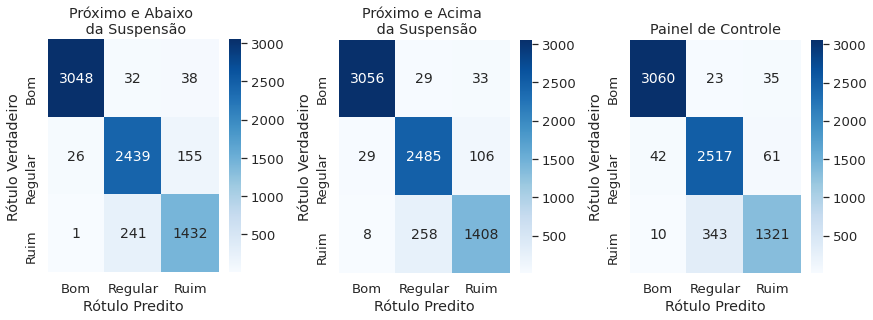
\includegraphics[width=1\textwidth]{figuras/fig_51.png}
  \fonte{Desenvolvido pelo autor.}
\end{figure}

Como podemos observar na \autoref{table:best_models_metrics_qualidade_superficie}, todas as classes de dados foram corretamente tratadas por todos os modelos sem haver viés, com valores acima de 80\%. Neste estudo, consideramos que o melhor modelo deve ser aquele que maximize tanto os VP quanto os VN, e minimize os FN e FP, de forma que a métrica \textit{f1-score} associa estes dois fatores. Analisando os valores, observamos que a rede CNN obteve os melhores resultados para praticamente todas as métricas em todas as classes, obtendo o melhor \textit{f1-score} em todas as classes. Sendo assim, consideramos o modelo baseado em CNN com janela de 500 amostras o melhor modelo para classificação de qualidade de superfície de pista, com valor de média entre \emph{experimentos por colocação} e \emph{experimentos por contexto} de 93,52\% para acurácia, 92,76\% para precisão, 91,52\% para \textit{recall} e 91,91\% para \textit{f1-score}. Na \autoref{fig:cnn_confusion_matrix_qualidade_superficie} é ilustrado a matriz confusão para o modelo baseado em CNN em cada ponto de coleta de dados.

